\documentclass{article}

\usepackage{arxiv}
\usepackage[utf8]{inputenc}
\usepackage[T1]{fontenc}
\usepackage{hyperref}
\usepackage{url}
\usepackage{booktabs}
\usepackage{amsfonts}
\usepackage{amsmath}
\usepackage{amssymb}
\usepackage{nicefrac}
\usepackage{microtype}
\usepackage{graphicx}
\usepackage[numbers]{natbib}
\usepackage{doi}
\usepackage{pgfplots}
\usepackage{tikz}
\usepackage{siunitx}
\usepackage{subcaption}
\usepackage{algorithm}
\usepackage{algpseudocode}
\usepackage{todonotes}
\usepackage{fontawesome5}
\usepackage{placeins}

\usetikzlibrary{arrows.meta, positioning, shapes.geometric, calc, decorations.markings, patterns, fit, backgrounds}
\usepgfplotslibrary{groupplots}
\pgfplotsset{compat=1.18}

\newcommand{\vect}[1]{\mathbf{#1}}
\newcommand{\mat}[1]{\mathbf{#1}}
\newcommand{\R}{\mathbb{R}}
\DeclareMathOperator*{\argmin}{argmin}
\DeclareMathOperator{\logsumexp}{LogSumExp}

\newcommand\figref{Figure~\ref}
\renewcommand\eqref{Equation~\ref}
\newcommand\tabref{Table~\ref}
\newcommand*{\secref}[1]{\hyperref[{#1}]{\S\ref*{#1}}}

\title{Differentiable Satellite Constellation Design via Relaxed Coverage and Revisit Objectives}

\author{
    \href{https://orcid.org/0000-0002-7227-4946}{
\includegraphics[scale=0.06]{orcid.pdf}\hspace{1mm}Shreeyam Kacker} \\
	Department of Aeronautics and Astronautics\\
	MIT\\
	\texttt{shreeyam@mit.edu}
    \And
    Kerri Cahoy \\
    Department of Aeronautics and Astronautics\\
    MIT\\
    \texttt{kcahoy@mit.edu}
}

\renewcommand{\headeright}{}
\renewcommand{\undertitle}{}
\renewcommand{\shorttitle}{Differentiable Constellation Design}

\hypersetup{
pdftitle={Differentiable Constellation Design via Relaxed Coverage and Revisit Objectives},
pdfsubject={astro-ph, cs.LG},
pdfauthor={Shreeyam Kacker, Kerri Cahoy},
pdfkeywords={satellite constellation, differentiable programming, orbit propagation, coverage optimization},
}

\begin{document}
\maketitle

\begin{abstract}
Satellite constellation design requires optimizing orbital parameters across multiple satellites to maximize mission specific metrics. For many types of mission, it is desirable to maximize coverage and minimize revisit gaps over ground targets. Existing approaches to constellation design either restrict the design space to symmetric parametric families such as Walker constellations, or rely on metaheuristic methods that require significant compute and many iterations. Gradient-based optimization has been considered intractable due to the non-differentiability of coverage and revisit metrics, which involve binary visibility indicators and discrete max operations. We introduce four continuous relaxations: soft sigmoid visibility, noisy-OR multi-satellite aggregation, leaky integrator revisit gap tracking, and LogSumExp soft-maximum, which when composed with the $\partial$SGP4 differentiable orbit propagator, yield a fully differentiable pipeline from orbital elements to mission-level objectives. We show that this scheme can recover Walker-Delta geometry from irregular initializations, and discovers elliptical Molniya-like orbits with apogee dwell over northern latitudes, from only gradients.
\end{abstract}

\noindent\textbf{Keywords:} satellite constellation design, differentiable programming, orbit propagation

\noindent\faGithub\hspace{0.5em}\url{https://github.com/shreeyam/differentiable_eo}

\section{Introduction}
\label{sec:introduction}

% Satellite constellation design---selecting orbital parameters for a fleet of satellites to optimize Earth observation performance---is a central problem in mission planning~\citep{wertz2011space}.
% For missions requiring responsive coverage of specific regions or targets, the design challenge is acute: the constellation must provide frequent revisit over non-uniform, mission-specific areas of interest while respecting orbital mechanics constraints.
% Applications range from disaster monitoring~\citep{paek_optimization_2019} and maritime domain awareness to agricultural surveillance and defense reconnaissance.
Designing satellite constellations is a fundamental problem in space mission design, across applications such as Earth Observation (EO), telecommunications, and navigation. The design space is high dimensional, with each spacecraft bringing up to six degrees of freedom corresponding to their orbital elements, and a wide range of often competing objectives to optimize over---for example, coverage and revisit over targets of interest, daytime illumination for optical payloads, and downlink contact time with ground stations.

Traditional approaches address this complexity in one of two ways.
Parametric families such as Walker Delta, Walker Star~\citep{walker_satellite_1984}, and Flower constellations~\citep{mortari_flower_2004} reduce the design space to a fixed set of parameters but are inherently symmetric, making them unable to capture non-uniform objectives.
Metaheuristic methods such as genetic algorithms can handle arbitrary objectives but require thousands to millions of simulator rollouts~\citep{paek_optimization_2019}.

For EO missions, the design problem has additional complexity---coverage and daytime revisit requirements may be non-uniform across ground targets, with additional constraints on data downlink. The combinatorial nature of the problem makes metaheuristic methods computationally expensive \citet{paek_optimization_2019}, with computational cost growing rapidly with the number of satellites and the number of free parameters.

Gradient-based optimization has been previously attempted constellation design, but with limited success. \citet{paek_optimization_2019} found the problem poorly conditioned for gradient-based methods, with difficulty even achieving convergence. Previous work has been limited by the non-differentiability of the computational graph, requiring finite difference approximations of gradients \cite{paek_optimization_2019}. Recent work by \citet{acciarini_closing_2025} addresses this gap by developing $\partial$SGP4, an end-to-end differentiable SGP4 orbit propagator. However, the coverage and revisit metrics themselves remain non-differentiable, due to requiring binary visibility indicators, Boolean OR operations, and max functions.

In this work we focus on constellation configuration: given a fixed fleet of $N$ satellites, assigning orbital elements to best meet mission-level coverage and revisit objectives. We make the following contributions:

\begin{enumerate}
    \item \textbf{Four continuous relaxations} that make coverage and revisit objectives differentiable: a soft sigmoid for visibility, a noisy-OR for multi-satellite aggregation, a leaky integrator for revisit gap tracking, and a LogSumExp soft-maximum for worst-case revisit (\figref{fig:relaxations}).
    \item \textbf{An end-to-end differentiable pipeline} from orbital elements to mission-level coverage metrics, composed with $\partial$SGP4~\citep{acciarini_closing_2025} and optimized with the AdamW optimizer (\figref{fig:pipeline}).
    \item \textbf{Demonstration on weighted target optimization}, recovering Molniya-like orbits for coverage over extreme latitudes (\secref{sec:experiments}).
\end{enumerate}

\paragraph{Paper organization.}
We review prior work on constellation design and differentiable physics simulation (\secref{sec:related_work}) before formulating the exact problem and introducing the relaxations required to make constellation configuration differentiable (\secref{sec:method}). We then conduct experiments on a toy problem, Walker-delta recovery from an irregular initialization, and weighted regional target optimization (\secref{sec:experiments}), benchmarking against tuned SA/GA/DE baselines with ablations isolating each design choice. We close (\secref{sec:conclusion}) with the scope of the configuration problem and the mission-driven constraints that fit naturally into the same method.

\begin{figure*}[h]
    \centering
    \includegraphics[width=.85\linewidth]{figures/overview.pdf}
    \caption{%
        Overview of end-to-end differentiable constellation optimization.
        \textbf{Top:} Starting from a constellation with irregularly spaced orbital planes and satellites, gradient optimization through the differentiable pipeline recovers a well-spaced constellation optimized for both coverage and revisit for a set of ground points.
        \textbf{Bottom:} Orbital parameters $\boldsymbol{\theta}_i$ are propagated through a differentiable orbit propagator~\citep{acciarini_closing_2025} and
        evaluated against a set of ground targets $\vect{g}_j$ to produce relaxed coverage and revisit metrics ($\tilde{C}$, $\tilde{\Delta}^{\max}$), which form a
        differentiable loss $\mathcal{L}$. Gradients
        $\nabla_{\boldsymbol{\theta}}\mathcal{L}$ flow back
        to the orbital parameters via reverse-mode automatic differentiation and are consumed by the optimizer to produce the next iterate.%
    }
    \label{fig:pipeline}
\end{figure*}

\section{Related Work}
\label{sec:related_work}

\subsection{Constellation Design and Optimization}

Parametric constellations significantly reduce the number of design parameters, with the Walker Delta pattern \citep{walker_satellite_1984} requiring only the number of planes, satellites per plane, and inclination. Flower constellations extend these ideas by using elliptical orbits to form specific ``harmonics'' in revisit rates to produce repeating ground tracks \citep{mortari_flower_2004}, allowing for directed coverage over a specific area. These parametric families are efficient but inherently symmetric, and cannot be tailored to non-uniform or mission-specific coverage requirements without breaking the symmetry assumptions that make them tractable.

For non-parametric design, previous work has relied primarily on metaheuristic methods.
\citet{paek_optimization_2019} uses genetic algorithms and simulated annealing to reconfigure constellations, optimizing for global coverage and regional revisit over five design variables, requiring approximately 2500 total evaluations through computationally expensive STK orbit simulations.
They also attempted gradient-based optimization via finite differences and found it ``extremely poorly conditioned,'' with convergence rarely achieved.
In a survey of 144 papers on constellation design, \citet{choo_survey_2024} finds that gradient methods appear as a design approach in only two of the surveyed articles, making it among the least common methods---ranking far behind genetic algorithms, simulated annealing, and analytical approaches.
Neither of the two entries actually uses analytic gradients.
The first, \citet{fraire_sparse_2020}, is labeled a gradient method but in fact uses a greedy neighbor search over discrete parameters (number of satellites, planes, inclination) with no gradients computed.
The second, \citet{abdelkhalik_optimization_2011}, pairs a genetic algorithm with a ``second-order gradient'' refinement step to cover ground sites under $J_2$ perturbations and explicitly notes that the fitness landscape contains numerous local minima that cause classical optimization methods to fail---but the gradient refinement is applied to a single-orbit subproblem rather than the multi-satellite design variables, so the overall design loop remains heuristic.
Separately, \citet{williams_rogers_optimal_2026} formulate constellation configuration as a collection of mixed-integer linear programs that select which satellites to activate from a pre-enumerated set of orbital slots, yielding provably optimal solutions for coverage and revisit objectives; however, the orbital slots and their underlying geometry (altitude, inclination, eccentricity) must be fixed a priori, so the method cannot discover improved orbit parameters.
We benchmark against SA/GA/DE baselines quantitatively in \secref{sec:baselines}.

\citet{hwang_large-scale_2014} demonstrates true gradient-based optimization of a satellite system through OpenMDAO (Open-Source Framework for Multidisciplinary Design, Analysis, and Optimization), optimizing a single satellite's subsystem design across seven coupled disciplines with over 25{,}000 design variables, with gradient computation made tractable with adjoint state methods. Their work utilizes gradient-based objectives combined with orbit-dependent parameters,  such as solar panel angles, battery sizing, and communication scheduling, to optimize a single spacecraft's operation. 

% This work differs in two respects: we use true analytical gradients through a complete computational graph rather than finite-difference approximations through a simulator, and we make the coverage and revisit objectives themselves differentiable via continuous relaxations rather than treating them as discrete metrics.

\subsection{Differentiable Physics and Simulation}

Differentiable programming~\citep{baydin_automatic_2018} allows for gradients to be obtained across domains even where forward models are complex but smooth. 
The benefits of differentiable programming have been made significantly more accessible through frameworks that perform automatic differentiation, such as PyTorch and JAX.
\citet{hu_difftaichi_2020} demonstrated differentiable physical simulators targeting robotics and fluid dynamics, and \citet{degrave_differentiable_2019} develops differentiable physics engines for contact-rich robotics.
For continuous relaxations applied to parameterized categorical distributions, Gumbel-Softmax reparameterization~\citep{jang_categorical_2017} is frequently used to compute analytic gradients.
\citet{kamra_gradient-based_2021} proves a coverage gradient theorem for spatial multi-resource coverage objectives, providing an estimator for the gradient that can be used for optimization of sensor placement, via spatial discretization and implicit boundary differentiation applied to 2D planar sensor networks.

In astrodynamics, \citet{acciarini_closing_2025} introduces $\partial$SGP4, a PyTorch reimplementation of the SGP4/SDP4 orbit propagation algorithm, which is forward mode differentiable.
\citet{naylor_dlite_2025} extends this direction by combining a JAX-based differentiable SGP4 propagator with Mitsuba~\citep{noauthor_mitsuba_nodate}, a differentiable renderer, to optimize trajectories for spacecraft-to-spacecraft inspection operations, demonstrating end-to-end forward-mode differentiation through orbit propagation chained with a rendering pipeline.

This work builds on $\partial$SGP4 by introducing differentiable coverage and revisit objectives that enable direct optimization of mission performance metrics.

\section{Method}
\label{sec:method}

\subsection{Problem Setup}
\label{sec:setup}

Consider a constellation of $N$ satellites, each parameterized by a two-line element (TLE) set.
For constellation geometry optimization at a fixed altitude, the free parameters per satellite are the inclination $\iota$, right ascension of the ascending node $\Omega$, and mean anomaly $\mathcal{M}$.
We fix the remaining TLE parameters (mean motion $n$, eccentricity $e \approx 0$, drag term $B^*$, and secular rates $\dot{n}$, $\ddot{n}$).

Given a grid of $M$ ground target points $\mathcal{G} = \{\vect{g}_1, \ldots, \vect{g}_M\}$ on the Earth's surface and a time horizon $[0, T]$ discretized into $K$ steps with spacing $\delta t = T/(K-1)$, we seek to maximize coverage and minimize the worst-case revisit gap.

\paragraph{Propagation.}
Each satellite's TLE elements are propagated through dSGP4~\citep{acciarini2024dsgp4} to produce position vectors $\vect{r}_i(t_k)$ in the True Equator Mean Equinox (TEME) reference frame.
These are rotated to the Earth-Centered Earth-Fixed (ECEF) frame via the Greenwich Mean Sidereal Time angle $\theta_{\text{GMST}}(t_k)$:
\begin{equation}
    \vect{r}_i^{\text{ECEF}}(t_k) = \mat{R}_z\bigl(\theta_{\text{GMST}}(t_k)\bigr) \, \vect{r}_i^{\text{TEME}}(t_k),
    \label{eq:teme_to_ecef}
\end{equation}
where $\mat{R}_z(\theta)$ is the standard rotation matrix about the $z$-axis.
This single-axis rotation is an approximation: the full TEME-to-ECEF transformation requires accounting for precession, nutation, and polar motion~\citep{vallado2006revisiting}.
For the \SI{24}{\hour} propagation horizons considered here, the precession-induced error is on the order of arcseconds, corresponding to sub-kilometre position offsets---negligible relative to the $\sim$\SI{2200}{\kilo\metre} ground footprint of a satellite at \SI{550}{\kilo\metre} altitude with \SI{10}{\degree} minimum elevation.
For longer horizons or higher-precision applications, the full IAU-2000/2006 transformation should be used.

\paragraph{Elevation angle.}
The elevation angle from ground point $\vect{g}_j$ to satellite $i$ at time $t_k$ is
\begin{equation}
    \alpha_{ij}(t_k) = \arcsin\left(\frac{(\vect{r}_i^{\text{ECEF}}(t_k) - \vect{g}_j) \cdot \hat{\vect{g}}_j}{\|\vect{r}_i^{\text{ECEF}}(t_k) - \vect{g}_j\|}\right),
    \label{eq:elevation}
\end{equation}
where $\hat{\vect{g}}_j = \vect{g}_j / \|\vect{g}_j\|$ is the local vertical unit vector at the ground point.
A satellite is conventionally visible when $\alpha_{ij} \geq \alpha_{\min}$, with $\alpha_{\min} = \SI{10}{\degree}$.

The challenge is that the visibility indicator $\mathbf{1}[\alpha_{ij}(t_k) \geq \alpha_{\min}]$, the Boolean OR over satellites, the revisit gap computation, and the worst-case maximum are all non-differentiable.
We address each in turn.

\subsection{Relaxation 1: Soft Visibility}
\label{sec:soft_visibility}

We replace the hard step function with a sigmoid (\figref{fig:relaxations}a):
\begin{equation}
    c_{ij}(t_k) = \sigma\!\left(\frac{\alpha_{ij}(t_k) - \alpha_{\min}}{\tau}\right), \quad \sigma(x) = \frac{1}{1 + e^{-x}},
    \label{eq:soft_visibility}
\end{equation}
where $\tau > 0$ controls the sharpness.
As $\tau \to 0$ this recovers the hard indicator; we use $\tau = \SI{2}{\degree}$, which provides a smooth transition zone of approximately $\pm\SI{6}{\degree}$ around the threshold while keeping the approximation tight.
This is analogous to the temperature-scaled softmax used in Gumbel-Softmax relaxations of discrete variables~\citep{jang2017categorical}.

\subsection{Relaxation 2: Noisy-OR Coverage Aggregation}
\label{sec:noisy_or}

For a ground point $\vect{g}_j$ at time $t_k$, we need to determine whether \emph{any} satellite provides coverage---a Boolean OR.
Treating each $c_{ij}(t_k)$ as an independent detection probability, the noisy-OR~\citep{pearl1988probabilistic} gives (\figref{fig:relaxations}b):
\begin{equation}
    C_j(t_k) = 1 - \prod_{i=1}^{N} \bigl(1 - c_{ij}(t_k)\bigr).
    \label{eq:noisy_or}
\end{equation}
This is smooth, monotonically increasing in each $c_{ij}$, and recovers the hard OR when all inputs are in $\{0, 1\}$.
It also naturally handles overlapping coverage: adding a satellite that already covers a point produces diminishing marginal gain, preventing the optimizer from clustering satellites.

The \emph{coverage fraction} over the full space-time grid is
\begin{equation}
    \bar{C} = \frac{1}{KM} \sum_{k=1}^{K} \sum_{j=1}^{M} C_j(t_k).
    \label{eq:coverage_fraction}
\end{equation}

\subsection{Relaxation 3: Leaky Integrator for Revisit Gaps}
\label{sec:leaky_integrator}

The revisit gap at a ground point is the time elapsed since the last coverage event.
Computing this requires identifying discrete transitions, which is non-differentiable.
We approximate it with a leaky integrator recurrence~\citep{gerstner2002spiking} (\figref{fig:relaxations}c):
\begin{equation}
    \Delta_j(t_k) = \bigl(\Delta_j(t_{k-1}) + \delta t\bigr) \cdot \bigl(1 - C_j(t_k)\bigr), \quad \Delta_j(t_0) = 0.
    \label{eq:leaky_integrator}
\end{equation}
When the point is covered ($C_j \approx 1$), the accumulated gap is multiplied by $\approx 0$, resetting it.
When the point is not covered ($C_j \approx 0$), the gap grows by $\delta t$.
This recurrence is fully differentiable and its maximum over time approximates the true worst-case revisit gap at each ground point.

\subsection{Relaxation 4: LogSumExp Soft-Maximum}
\label{sec:logsumexp}

The worst-case revisit gap at ground point $\vect{g}_j$ is $\max_k \Delta_j(t_k)$, which has zero gradients almost everywhere.
We replace it with the LogSumExp smooth maximum~\citep{boyd2004convex} (\figref{fig:relaxations}d):
\begin{equation}
    \widetilde{\Delta}_j^{\max} = \tau_r \cdot \log\!\left(\sum_{k=1}^{K} \exp\!\left(\frac{\Delta_j(t_k)}{\tau_r}\right)\right),
    \label{eq:logsumexp}
\end{equation}
where $\tau_r = \SI{30}{\minute}$.
This satisfies $\max_k \Delta_j(t_k) \leq \widetilde{\Delta}_j^{\max} \leq \max_k \Delta_j(t_k) + \tau_r \log K$, providing a controllable upper bound.
The mean worst-case revisit across all ground points is
\begin{equation}
    \bar{\Delta}^{\max} = \frac{1}{M} \sum_{j=1}^{M} \widetilde{\Delta}_j^{\max}.
    \label{eq:mean_revisit}
\end{equation}

\begin{figure}[t]
    \centering
    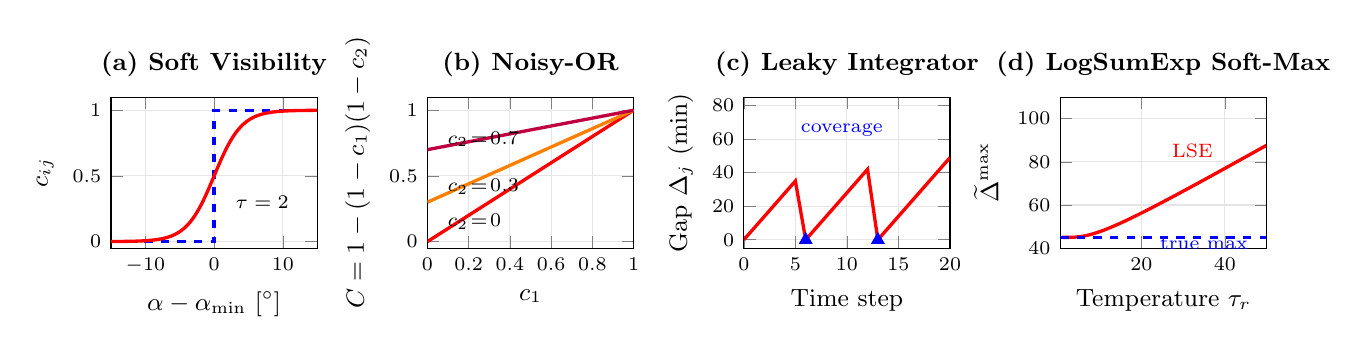
\begin{tikzpicture}
\begin{groupplot}[
    group style={
        group size=4 by 1,
        horizontal sep=1.4cm,
    },
    width=4.2cm, height=3.5cm,
    grid=major,
    grid style={gray!20},
    tick label style={font=\scriptsize},
    label style={font=\small},
    title style={font=\small\bfseries, yshift=-2pt},
]

% (a) Soft sigmoid
\nextgroupplot[
    title={(a) Soft Visibility},
    xlabel={$\alpha - \alpha_{\min}$ [\si{\degree}]},
    ylabel={$c_{ij}$},
    xmin=-15, xmax=15,
    ymin=-0.05, ymax=1.1,
    domain=-15:15,
    samples=100,
]
% Hard step
\addplot[blue, very thick, dashed] coordinates {(-15,0) (0,0) (0,1) (15,1)};
% Soft sigmoid tau=2
\addplot[red, very thick] {1/(1+exp(-x/2))};
\node[font=\scriptsize] at (axis cs:7,0.3) {$\tau=2$};

% (b) Noisy-OR
\nextgroupplot[
    title={(b) Noisy-OR},
    xlabel={$c_1$},
    ylabel={$C = 1 - (1-c_1)(1-c_2)$},
    xmin=0, xmax=1,
    ymin=-0.05, ymax=1.1,
    domain=0:1,
    samples=50,
]
\addplot[red, very thick] {1-(1-x)*(1-0.0)};
\addplot[orange, very thick] {1-(1-x)*(1-0.3)};
\addplot[purple, very thick] {1-(1-x)*(1-0.7)};
\node[font=\scriptsize, anchor=west] at (axis cs:0.05,0.15) {$c_2\!=\!0$};
\node[font=\scriptsize, anchor=west] at (axis cs:0.05,0.42) {$c_2\!=\!0.3$};
\node[font=\scriptsize, anchor=west] at (axis cs:0.05,0.78) {$c_2\!=\!0.7$};

% (c) Leaky integrator
\nextgroupplot[
    title={(c) Leaky Integrator},
    xlabel={Time step},
    ylabel={Gap $\Delta_j$ (min)},
    xmin=0, xmax=20,
    ymin=-5, ymax=85,
]
% Simulated gap signal: grows linearly, resets at coverage events
\addplot[red, very thick] coordinates {
    (0,0) (1,7) (2,14) (3,21) (4,28) (5,35)
    (6,0) (7,7) (8,14) (9,21) (10,28) (11,35) (12,42)
    (13,0) (14,7) (15,14) (16,21) (17,28) (18,35) (19,42) (20,49)
};
% Coverage events
\addplot[blue, only marks, mark=triangle*, mark size=2.5pt] coordinates {(6,0) (13,0)};
\node[font=\scriptsize, blue] at (axis cs:9.5,65) {coverage};

% (d) LogSumExp
\nextgroupplot[
    title={(d) LogSumExp Soft-Max},
    xlabel={Temperature $\tau_r$},
    ylabel={$\widetilde{\Delta}^{\max}$},
    xmin=0.5, xmax=50,
    ymin=40, ymax=110,
    domain=1:50,
    samples=50,
]
% For values [20, 45, 30], true max = 45
\addplot[red, very thick] {x * ln(exp(20/x) + exp(45/x) + exp(30/x))};
\addplot[blue, very thick, dashed] coordinates {(0.5,45) (50,45)};
\node[font=\scriptsize, blue] at (axis cs:35,42) {true max};
\node[font=\scriptsize, red, anchor=west] at (axis cs:25,85) {LSE};

\end{groupplot}
\end{tikzpicture}

    \caption{The four continuous relaxations.  \textbf{(a)} Soft sigmoid replaces the hard visibility threshold.  \textbf{(b)} Noisy-OR aggregates coverage across satellites.  \textbf{(c)} Leaky integrator tracks the revisit gap as a differentiable recurrence.  \textbf{(d)} LogSumExp approximates the worst-case (maximum) revisit gap.}
    \label{fig:relaxations}
\end{figure}

\subsection{Combined Objective}
\label{sec:objective}

The total loss combines coverage maximization with revisit minimization:
\begin{equation}
    \mathcal{L}(\vect{x}) = -\bar{C} + \lambda \, \bar{\Delta}^{\max},
    \label{eq:loss}
\end{equation}
where $\vect{x} = \{\iota_i, \Omega_i, \mathcal{M}_i\}_{i=1}^{N}$ collects all free orbital parameters and $\lambda$ is a weighting coefficient.
For non-uniform objectives, the sums over ground points can be replaced with weighted sums over a discrete target set (\secref{sec:weighted}).

\subsection{Tightness of the Composed Relaxation}
\label{sec:tightness}

Each of the four relaxations is individually tight: the soft sigmoid recovers the hard step as $\tau \to 0$; the noisy-OR is exact when its inputs are binary; the leaky integrator is exact when coverage is in $\{0, 1\}$; and the LogSumExp satisfies $\max_k x_k \leq \text{LSE} \leq \max_k x_k + \tau_r \log K$.
However, the \emph{composition} of these relaxations does not inherit these guarantees, because each relaxation receives the soft output of the previous one rather than the binary values for which it was designed.

The interaction introduces two competing biases:

\paragraph{Phantom coverage (gap shortening).}
The soft sigmoid assigns nonzero coverage $c_{ij} > 0$ to satellites slightly \emph{below} the visibility threshold ($\alpha_{ij} < \alpha_{\min}$).
This phantom coverage propagates through the noisy-OR and partially resets the leaky integrator, producing gaps that are \emph{shorter} than the true discrete gaps.
For example, a satellite at $\alpha = \alpha_{\min} - 2\tau$ contributes $c_{ij} \approx 0.12$, which the leaky integrator treats as a partial coverage event.

\paragraph{Incomplete reset (gap lengthening).}
Conversely, a satellite well above the threshold produces $c_{ij} \approx 0.99$, not exactly 1.
The leaky integrator retains a fraction $(1 - C_j) \approx 0.01$ of the accumulated gap at each coverage event.
Over time, this residual prevents the gap from fully resetting, producing relaxed gaps that are \emph{longer} than the true gaps during sustained coverage.
The LogSumExp adds a further upward bias of at most $\tau_r \log K$.

These effects compete: phantom coverage shortens gaps near the visibility boundary, while incomplete resets and the LogSumExp overestimate lengthen them.
The net bias depends on the specific geometry and is neither a guaranteed upper nor lower bound on the true objective.

For optimization, the critical question is not whether the relaxed loss equals the true loss, but whether the two have similar \emph{optima}.
We validate this empirically in \secref{sec:relaxation_quality} by computing the hard (discrete) coverage and revisit metrics at the optimizer's solution and comparing them to the relaxed values.
The relaxation temperatures $\tau$ and $\tau_r$ control the trade-off: smaller values tighten the approximation but sharpen the gradients, potentially destabilizing optimization.
A temperature annealing schedule---starting with large temperatures for a smooth landscape and progressively tightening---could mitigate this trade-off, though we leave this to future work.

\subsection{Optimization}
\label{sec:optimization}

The full computational graph is:
\begin{equation}
    \underbrace{\vect{x}_i}_{\text{TLE}} \xrightarrow{\text{dSGP4}} \underbrace{\vect{r}_i(t)}_{\text{TEME}} \xrightarrow{\text{GMST}} \underbrace{\vect{r}_i^{\text{ECEF}}(t)}_{\text{ECEF}} \xrightarrow{\text{Eq.~\ref{eq:elevation}}} \alpha_{ij}(t) \xrightarrow{\text{Eqs.~\ref{eq:soft_visibility}--\ref{eq:mean_revisit}}} \mathcal{L}.
    \label{eq:pipeline}
\end{equation}
Every operation is implemented in PyTorch~\citep{paszke2019pytorch}, so $\nabla_{\vect{x}_i} \mathcal{L}$ is computed via reverse-mode automatic differentiation.

A practical complication is that $\partial$SGP4's \texttt{initialize\_tle} function rebuilds the computation graph from scratch at each call, producing a new ephemeral tensor for each satellite's elements.
Standard optimizers like \texttt{torch.optim.Adam} track specific tensor objects and would lose their momentum state.
We solve this by maintaining persistent parameter tensors that Adam tracks, and copying gradients from dSGP4's ephemeral tensors after each backward pass:
\begin{equation}
    \vect{p}_i.\text{grad} \leftarrow \text{clip}\bigl(\nabla_{\vect{x}_i^{\text{eph}}} \mathcal{L},\ [-5, 5]\bigr) \odot \vect{m},
    \label{eq:grad_copy}
\end{equation}
where $\vect{p}_i$ is the persistent parameter tensor, $\vect{x}_i^{\text{eph}}$ is dSGP4's ephemeral tensor, and $\vect{m} \in \{0,1\}^9$ is a binary mask that zeroes gradients for fixed parameters (altitude, eccentricity, drag).
Adam then steps on $\vect{p}_i$, and the updated values are written back to the TLE object before the next iteration.

The per-iteration cost is $\mathcal{O}(NKM)$: $N$ satellite propagations over $K$ time steps, each evaluated against $M$ ground points.

\section{Experiments}
\label{sec:experiments}

We evaluate the framework on three experiments: a toy problem validating gradient correctness, a uniform-coverage baseline that recovers known-optimal geometries, and a weighted target optimization on a problem class where parametric families fail.

\subsection{Common Setup}
\label{sec:common_setup}

All experiments use $\partial$SGP4~\citep{acciarini_closing_2025} for orbit propagation with PyTorch autograd for gradient computation, and AdamW with learning rate $\eta = 10^{-2}$  for optimization.
Circular orbits are assumed and held stationary by zeroing the mean-motion gradient.
The minimum elevation angle for all ground points is $\alpha_{\min} = \SI{10}{\degree}$.
As discussed in \secref{sec:tightness}, we use separate sigmoid temperatures for coverage and revisit: the coverage temperature $\tau_{\text{cov}}$ controls gradient smoothness, while a tighter revisit temperature $\tau_{\text{rev}}$ prevents the leaky integrator from being gamed by phantom coverage.
To select these quantities and the remaining hyperparameters ($\beta$, $\lambda$), we optimize a 24-satellite constellation from four initializations ranging from well-spread to heavily clustered, then grid-search over temperature and weight combinations to find settings that correctly rank the resulting solutions by their hard metrics.
This calibration confirms that $\tau_{\text{cov}} \gg \tau_{\text{rev}}$ is required for correct ranking, though in practice we favor slightly softer values that improve convergence at the expense of absolute correctness (Appendix~\ref{app:hyperparam_grid}).
Coverage and revisit metrics are evaluated over a \SI{24}{\hour} propagation horizon discretized into $K = 240$ time steps on a ground grid of $36 \times 72 = 2592$ points spanning $\pm\SI{70}{\degree}$ latitude.
In each experiment the satellite count $N$ and plane structure are fixed ahead of time and chosen to match the intended comparison geometry (e.g.\ Walker 24/6/1 in \secref{sec:uniform}): this paper addresses the configuration problem, not the sizing problem.
Specific relaxation parameters, optimizer settings, and revisit weight $\lambda$ vary per experiment and are stated in each subsection.

\subsection{Experiment 1: Toy Problem}
\label{sec:toy}
    
To validate that the relaxed objectives produce correct gradients and results, we consider the simplest non-trivial constellation design problem: two satellites in a single orbital plane at \SI{550}{\kilo\metre} altitude with inclination fixed at \SI{60}{\degree} and RAAN fixed at \SI{0}{\degree}, optimizing only their mean anomalies $\mathcal{M}_1$ and $\mathcal{M}_2$.
We use relaxation parameters $\tau_{\text{cov}} = \SI{5}{\degree}$, $\tau_{\text{rev}} = \SI{2}{\degree}$, $\beta = \SI{10}{\minute}$, $\lambda = 2.0$, and AdamW with learning rate $\eta = 10^{-2}$.

The optimal solution is known analytically: the two satellites should be separated by \SI{180}{\degree} in mean anomaly to maximize coverage and revisit rate within the shared orbital plane.
This reduces the problem to two free parameters, allowing the full loss landscape to be visualized.

\paragraph{Loss landscape.}
We evaluate both the relaxed loss and hard (discrete) metrics on a dense grid over $(\mathcal{M}_1, \mathcal{M}_2) \in [0, 360)^2$\SI{}{\degree}.  
\figref{fig:toy_landscape} shows the resulting landscapes.
Both landscapes exhibit a clear global minimum along the anti-diagonal $|\mathcal{M}_1 - \mathcal{M}_2| = \SI{180}{\degree}$, with no local minima.
The relaxed landscape is visibly smoother than the hard landscape while preserving the same basin structure, confirming that the relaxations provide a smooth surface amenable to gradient descent without significantly distorting the underlying objective.

\paragraph{Gradient descent trajectory.}
Starting from $\mathcal{M}_1 = \SI{179}{\degree}$, $\mathcal{M}_2 = \SI{181}{\degree}$ the optimizer converges to $|\mathcal{M}_1 - \mathcal{M}_2| \approx \SI{180}{\degree}$ within 800 iterations.
The trajectory (overlaid in white on \figref{fig:toy_landscape}) follows the gradient field smoothly toward the minimum without oscillation.
This validates that the composed relaxations produce well-behaved gradients---a prerequisite for the higher-dimensional experiments that follow.

\begin{figure}[!htb]
    \centering
    
\includegraphics[width=\textwidth]{figures/exp1_gradient_validation.pdf}
    \caption{Two-satellite mean anomaly optimization. \textbf{Top:} relaxed metrics. \textbf{Bottom:} hard metrics. The optimizer (white line) converges to the optimal \SI{180}{\degree} separation. The relaxed landscape preserves the basin structure of the hard landscape while providing smooth gradients.}
    \label{fig:toy_landscape}
\end{figure}

\subsection{Experiment 2: Uniform Coverage Baseline}
\label{sec:uniform}

We now apply our gradient-based scheme to a well-understood uniform coverage problem. We optimize $N = 24$ satellites in 6 orbital planes (4 per plane) with inclination fixed at \SI{60}{\degree}.
RAAN and mean anomaly are free, with RAAN shared within each plane, yielding $6 + 24 = 30$ effective degrees of freedom.

\paragraph{Initial configuration.}
We deliberately initialize the constellation with irregular RAAN offsets $[0, 30, 120, 200, 210, 300]$\SI{}{\degree} far from uniform spacing, and random mean anomalies. The classical Walker-delta $24/6/1$ pattern uses \SI{60}{\degree} RAAN spacing.

\paragraph{Results.}
Over 1000 iterations, the optimizer recovers near-uniform RAAN spacing from the irregular initialization, approaching the Walker-delta geometry without domain-specific inductive biases.
\tabref{tab:uniform_results} summarizes the metrics; \figref{fig:convergence} shows convergence, spatial coverage redistribution, and final RAAN/MA configuration space.

\begin{table}[!htb]
\centering
\caption{Recovery of Walker Delta constellation through gradient optimization of randomly initialized 24-satellite constellation ($6 \times 4$), 1000 iterations, \SI{550}{\kilo\metre} fixed altitude, inclination fixed at \SI{60}{\degree}.}
\label{tab:uniform_results}
\begin{tabular}{lrrr}
\toprule
\textbf{Metric} & \textbf{Initial} & \textbf{Optimized} & \textbf{Walker 24/6/1} \\
\midrule
Hard coverage [\%] & 32.41 & 40.34 & 40.33 \\
Hard mean max revisit [min] & 136.2 & 48.0 & 48.0 \\
\midrule
Soft coverage [\%] & 41.86 & 50.32 & 50.32 \\
Soft mean max revisit [min] & 127.5 & 73.5 & 73.5 \\
\bottomrule
\end{tabular}
\end{table}

\begin{figure}[!htb]
    \centering
    \begin{minipage}[t]{0.48\textwidth}
        \centering
        \includegraphics[width=\textwidth]{figures/exp2_convergence.pdf}\\[-2pt]
        {\small (a) Convergence}
    \end{minipage}%
    \hfill
    \begin{minipage}[t]{0.48\textwidth}
        \centering
        \includegraphics[width=\textwidth]{figures/exp2_raan_ma.pdf}\\[-2pt]
        {\small (b) RAAN vs mean anomaly}
    \end{minipage}
    \caption{Walker recovery experiment. \textbf{(a)} Convergence of coverage and revisit over 1000 iterations, with Walker 24/6/1 reference (dashed). \textbf{(b)} RAAN vs mean anomaly trajectories (hollow = initial, solid = optimized, stars = Walker). The optimizer recovers Walker-equivalent geometry (in rotational symmetry) from an irregular initialization.}
    \label{fig:convergence}
\end{figure}

\paragraph{Loss landscape.}
To investigate the structure of the loss landscape, we visualize it using per-trajectory PCA~\citep{li_visualizing_2018}: for each of the four initializations from the hyperparameter calibration (Appendix~\ref{app:hyperparam_grid}), we project the optimization trajectory onto its two principal components and evaluate the loss on that 2D slice.
\figref{fig:landscape} shows smooth basins in all four cases, confirming that the relaxations produce a landscape amenable to gradient descent. However, the global view reveals multi-modal structure: the clustered initializations converge to distinct local minima with worse hard metrics than the well-spread ones, indicating that initialization still matters despite the smooth local landscape.

\begin{figure*}[!htb]
    \centering
    
\includegraphics[width=\textwidth]{figures/exp3_loss_landscape.pdf}
    \caption{Loss landscape visualization~\citep{li_visualizing_2018}. \textbf{Left:} global view along random directions. \textbf{Columns 2--5:} per-trajectory PCA slices (white line = optimizer path). \textbf{Top/bottom:} relaxed and hard loss, respectively. Per-trajectory views show smooth basins; the global view reveals multi-modal structure.}
    \label{fig:landscape}
\end{figure*}

\subsection{Experiment 3: Regional Target Optimization}
\label{sec:weighted}

The primary advantage of gradient-based constellation optimization over parametric families is the ability to handle non-uniform, mission-specific objectives.
We demonstrate this by optimizing a small constellation for coverage and revisit over Europe---a problem that Walker constellations cannot address by construction.

\paragraph{Setup.}
We sample 500 ground targets from European country boundaries (GeoJSON), weighted by $\cos(\text{lat})$ to correct for area distortion.
The constellation consists of 4 satellites in 2 orbital planes (2 per plane).
Unlike Experiment~2, we free all orbital geometry parameters: inclination ($\iota \in [30, 90]$\SI{}{\degree}), RAAN, mean anomaly, argument of perigee, and orbital shape.
To allow the optimizer to explore eccentric orbits without producing unphysical perigee altitudes, we reparameterize eccentricity and altitude jointly as (perigee altitude, excess altitude), where perigee $\in [400, 600]$\SI{}{\kilo\metre} and excess $\in [0, 1500]$\SI{}{\kilo\metre}, guaranteeing perigee $\geq$ \SI{400}{\kilo\metre} by construction.
Inclination, RAAN, eccentricity, argument of perigee, and altitude are shared within each plane; mean anomaly is free per satellite, giving 12 effective degrees of freedom.
We use $\lambda = 1.0$, and run for 3000 iterations.

\paragraph{Results.}
Starting from a Walker-like circular initialization at \SI{550}{\kilo\metre}, the optimizer discovers a qualitatively different geometry (\tabref{tab:weighted_results}).
Both planes converge to highly elliptical orbits ($e \approx 0.40$) with argument of perigee $\omega \approx \SI{270}{\degree}$, placing apogee over the northern hemisphere where the satellite dwells longest.
The resulting orbits have perigee $\approx$ \SI{685}{\kilo\metre} and apogee $\approx$ \SI{10000}{\kilo\metre}---a Molniya-class highly elliptical orbit discovered entirely from gradients, with no domain-specific heuristics.
The inclination converges to $\sim$\SI{63}{\degree}--\SI{65}{\degree}, near the critical inclination (\SI{63.4}{\degree}) at which $J_2$ perturbations do not precess the argument of perigee.

The optimized constellation achieves 99.3\% coverage and 3.7~min mean revisit over Europe, compared to 10.0\% coverage and 247.5~min for a Walker 4/2/1 baseline (\tabref{tab:weighted_results}).
The comparison is not between equal orbit regimes: the Walker baseline is constrained to circular LEO while the optimizer is free to explore eccentric orbits. The result demonstrates that, given this freedom, the optimizer escapes the LEO basin and discovers a qualitatively different and far more effective geometry for regional coverage.

\figref{fig:europe_density} shows the visibility density (number of timesteps each ground bin is within \SI{10}{\degree} elevation of any satellite).
The optimized constellation concentrates nearly all coverage in the northern hemisphere over Europe, while the Walker baseline distributes coverage uniformly but achieves far less density.
The orbital period of $\sim$\SI{210}{\minute} produces approximately 7 revolutions per sidereal day, creating a near-resonant repeating ground track.

\begin{table}[!htb]
\centering
\caption{Regional target optimization: 4 satellites (2 planes $\times$ 2), 3000 iterations, all orbital geometry parameters free with coupled perigee/apoapsis constraints.}
\label{tab:weighted_results}
\begin{tabular}{lrr}
\toprule
\textbf{Metric} & \textbf{Walker 4/2/1} & \textbf{Optimized} \\
\midrule
Hard coverage [\%] & 9.97 & 99.25 \\
Hard mean max revisit [min] & 247.5 & 3.7 \\
Soft coverage [\%] & 12.37 & 97.99 \\
Soft mean max revisit [min] & 208.9 & 54.9 \\
\bottomrule
\end{tabular}
\end{table}

\begin{table}[!htb]
\centering
\caption{Per-plane orbital geometry discovered by the optimizer for the Europe target set. Both planes converge to eccentric, Molniya-like orbits with apogee over the northern hemisphere ($\omega \approx \SI{270}{\degree}$). The Walker baseline uses circular orbits at \SI{550}{\kilo\metre}.}
\label{tab:exp3_geometry}
\begin{tabular}{lrrrrr}
\toprule
& $\iota$ \textbf{[deg]} & $\Omega$ \textbf{[deg]} & $e$ & $\omega$ \textbf{[deg]} & \textbf{Perigee / Apogee [km]} \\
\midrule
Plane 0 & 62.6 & 336.6 & 0.398 & 276.2 & 685 / 10011 \\
Plane 1 & 65.3 & 155.6 & 0.402 & 266.5 & 687 / 10193 \\
\midrule
Walker (all) & 60.0 & uniform & 0.001 & --- & 550 / 550 \\
\bottomrule
\end{tabular}
\end{table}

\begin{figure}[htbp]
    \centering
    \includegraphics[width=0.48\textwidth]{figures/exp3_convergence.pdf}
    \caption{Convergence of the Europe target optimization over 3000 iterations. The optimizer rapidly improves both coverage and revisit over the Walker baseline (dashed).}
    \label{fig:exp3_convergence}
\end{figure}

\begin{figure}[!htb]
    \centering
    \includegraphics[width=.9\textwidth]{figures/exp3_groundtrack_optimized.pdf}\\[2pt]
    {\small (a) Optimized for Europe}\\[8pt]
    \includegraphics[width=.9\textwidth]{figures/exp3_groundtrack_walker.pdf}\\[2pt]
    {\small (b) Walker 4/2/1 baseline}
    \caption{Visibility density over \SI{24}{\hour}. \textbf{(a)} The optimized constellation concentrates coverage over Europe via eccentric orbits with apogee dwell over northern latitudes. \textbf{(b)} The Walker baseline distributes coverage uniformly but achieves far less density over the target region.}
    \label{fig:europe_density}
\end{figure}

\subsection{Comparison to Baseline Methods}
\label{sec:baselines}

Constellation design in prior work is typically posed as a black-box optimisation over design variables, handled either by population heuristics (simulated annealing, genetic algorithms) or off-the-shelf gradient-free libraries.
We benchmark our differentiable pipeline against three such baselines on the Walker recovery testbed of \secref{sec:uniform}: 24 satellites in a $6 \times 4$ arrangement at \SI{550}{\kilo\metre}, inclination fixed at \SI{60}{\degree}, and the same irregular-RAAN initialisation.
The decision vector has 30 continuous variables (six per-plane RAANs and 24 per-satellite mean anomalies).

\paragraph{Baselines.}
We compare against simulated annealing (SA), a genetic algorithm (GA), and differential evolution (DE), all applied to the same fitness $J = -C + \lambda \Delta^{\max}$ (with $\lambda = 0.1$ as in \secref{sec:uniform}), computed directly from the \emph{hard} coverage and revisit metrics of \eqref{eq:coverage_fraction_hard} and \eqref{eq:mean_revisit_hard}---the baselines do not see the relaxed objective.
SA and GA follow the constellation-design formulations used in prior heuristic work~\citep{paek_optimization_2019} with standard tuning: SA uses a probe-calibrated temperature schedule (\SI{80}{\percent} initial / \SI{1}{\percent} final acceptance, geometric cooling) and an adaptive step size targeting the Vanderbilt--Louie rate of $0.44$; GA uses tournament selection (size 3), uniform crossover, and Gaussian mutation with $\sigma$ annealed from $\SI{30}{\degree}$ to $\SI{5}{\degree}$.
DE uses the TwoPointsDE implementation from nevergrad~\citep{rapin_nevergrad_2018}.
All three baselines warm-start from the same irregular-RAAN configuration as the gradient run.
Each is run for 5 seeds with a budget of 4050 function evaluations (4000 main evaluations plus the 50-evaluation probe that SA uses to calibrate its temperature schedule, matched across methods); the gradient pipeline uses 1000 iterations of the relaxed objective.

\begin{table}[!htb]
\centering
\caption{Final hard metrics on the Walker recovery testbed. The gradient pipeline recovers the Walker reference exactly in 1000 iterations; the three black-box baselines plateau well short of it even with roughly four times the evaluation budget and best-of-5 seed selection.}
\label{tab:baselines}
% Manually generated from experiments/exp2_baselines.py (5 seeds, 4050 evals each: 4000 main + 50-eval SA probe, matched across methods)
% Range is min--max across seeds; the best side of each range is bolded
% (highest coverage, lowest revisit).
\begin{tabular}{lrr}
\toprule
\textbf{Method} & \textbf{Hard coverage [\%]} & \textbf{Hard mean worst-case revisit [min]} \\
\midrule
Walker 24/6/1 reference & 40.33 & 48.0 \\
Gradient (ours, 1000 iters) & \textbf{40.34} & \textbf{48.0} \\
\midrule
\multicolumn{3}{l}{\emph{Black-box baselines (4000 iters, range over 5 seeds):}} \\
\quad Simulated annealing       & 34.33--\textbf{36.54} & \textbf{73.9}--80.5 \\
\quad Genetic algorithm          & 37.83--\textbf{38.69} & \textbf{60.3}--62.2 \\
\quad TwoPointsDE~\citep{rapin_nevergrad_2018} & 35.77--\textbf{37.44} & \textbf{68.5}--76.1 \\
\bottomrule
\end{tabular}

\end{table}

\figref{fig:baselines_conv} plots convergence for the best-fitness seed of each method against function evaluations; the $x = 0$ values carry the common bad initialisation forward by zero-order hold.
The differentiable pipeline reaches the Walker reference (\SI{40.3}{\percent} coverage, \SI{48}{\minute} revisit) at roughly 750 evaluations and is flat thereafter.
Among the heuristics, GA performs best (\SI{60.3}{\min} revisit, best seed), followed by DE (\SI{68.5}{\min}) and SA (\SI{73.9}{\min}); in our experiments with these tuned baselines, none come within \SI{12}{\minute} of Walker revisit within the \num{4050}-evaluation budget.
GA's edge over DE on this problem is attributable to its uniform crossover and $\bmod\,\SI{360}{\degree}$ wrap, which respect the cyclic nature of RAAN and mean anomaly; DE's Euclidean-space perturbations do not.\footnote{The nevergrad NGOpt meta-selector chooses CMA-ES with box constraints at this budget and dimension; we found it plateaus earlier than TwoPointsDE and report the stronger of the two.}
The gap between the gradient pipeline and all three baselines is consistent with the information-per-evaluation argument: each gradient step uses a 30-dimensional descent direction obtained by autodiff through the relaxed objective, whereas the baselines receive a single scalar per evaluation.

\begin{figure}[!htb]
    \centering
    \begin{minipage}[t]{0.49\linewidth}\centering
        \includegraphics[width=\textwidth]{figures/exp2_method_comparison_coverage.pdf}\\[-2pt]
        {\small (a) Hard coverage}
    \end{minipage}\hfill
    \begin{minipage}[t]{0.49\linewidth}\centering
        \includegraphics[width=\textwidth]{figures/exp2_method_comparison_revisit.pdf}\\[-2pt]
        {\small (b) Hard mean worst-case revisit}
    \end{minipage}
    \caption{Convergence of the differentiable optimiser (teal, Exp 2 baseline) against three black-box baselines on the Walker recovery testbed. Best-of-5 seeds shown per method; evaluation $0$ shares the common irregular-RAAN initialisation by zero-order hold, and the Walker reference is dotted grey. The gradient pipeline matches Walker at ${\sim}750$ evaluations; the heuristics plateau above Walker revisit even with roughly four times the budget.}
    \label{fig:baselines_conv}
\end{figure}

\subsection{Ablations}
\label{sec:ablations}

To isolate the design choices behind the relaxed pipeline, we re-run the Walker recovery testbed of \secref{sec:uniform} (24 satellites, $6 \times 4$, inclination fixed at \SI{60}{\degree}, RAAN and mean anomaly free, irregular RAAN init, 1000 iterations) under five controlled perturbations.
Constellation, ground grid, propagation horizon, and optimizer are held fixed; only the ablated knob varies.
Each row of \tabref{tab:ablations} reports the final hard coverage and mean worst-case revisit; the Walker 24/6/1 reference is included for calibration.

\begin{table}[!htb]
\centering
\caption{Design-choice ablations on the Walker recovery testbed (\secref{sec:uniform}, 24 satellites, 1000 iterations, hard metrics evaluated at the final step). Default settings (used elsewhere unless ablated) are $\lambda = 0.1$, $\tau_{\text{cov}} = \tau_{\text{rev}} = \SI{2}{\degree}$, $\beta = \SI{10}{\minute}$.}
\label{tab:ablations}
% Auto-generated by experiments/exp4_ablations.py
\begin{tabular}{lrr}
\toprule
\textbf{Setting} & \textbf{Hard coverage [\%]} & \textbf{Hard mean worst-case revisit [min]} \\
\midrule
Walker 24/6/1 reference / Exp 2 defaults & 40.34 & 48.0 \\
\midrule
(a) Coverage only ($\lambda = 0$) & 40.76 & 126.7 \\
(a) Revisit only ($-\tilde{C}$ dropped) & 40.34 & 48.0 \\
(b) Split $\tau$ ($\tau_{\text{cov}}=3^{\circ}$, $\tau_{\text{rev}}=1^{\circ}$) & 39.04 & 54.9 \\
(b) Split $\tau$ inverted ($\tau_{\text{cov}}=1^{\circ}$, $\tau_{\text{rev}}=3^{\circ}$) & 40.11 & 58.3 \\
(c) $\lambda = 0.01$ & 40.06 & 59.8 \\
(c) $\lambda = 1.0$ & 40.34 & 47.9 \\
(d) $\beta = 1$ min & 38.58 & 55.3 \\
(d) $\beta = 100$ min & 40.08 & 68.9 \\
(e) Random RAAN+MA init, $n=10$ & 39.73 $\pm$ 0.46 (38.82--40.34) & 61.7 $\pm$ 4.7 (47.8--64.1) \\
\bottomrule
\end{tabular}

\end{table}

\paragraph{(a) Loss composition.}
Coverage-only preserves Walker-level coverage (\SI{40.8}{\percent}) but leaves revisit at \SI{126.7}{\minute}---over \SI{2.6}{\times} the Walker baseline---because the loss never penalises long gaps.
In contrast, revisit-only and the full combined loss both converge to the Walker-equivalent solution (\SI{40.3}{\percent} coverage, \SI{48.0}{\minute} revisit): once satellites are spaced to minimise revisit, the coverage term contributes only a small residual gradient, so the two are effectively equivalent on this testbed.
The combined form remains load-bearing on problems where clustering is a valid local minimum of the revisit objective (\secref{sec:weighted}); here it confirms that adding the coverage term does no harm.

\paragraph{(b) Sigmoid temperature.}
We compare the shared baseline ($\tau_{\text{cov}} = \tau_{\text{rev}} = \SI{2}{\degree}$, used in \secref{sec:uniform}) against the split values calibrated in Appendix~\ref{app:hyperparam_grid} ($\tau_{\text{cov}} = \SI{3}{\degree}$, $\tau_{\text{rev}} = \SI{1}{\degree}$) and the inverse split ($\tau_{\text{cov}} = \SI{1}{\degree}$, $\tau_{\text{rev}} = \SI{3}{\degree}$).
The shared setting recovers Walker (\SI{40.3}{\percent}, \SI{48.0}{\minute}); both split variants underperform (\SI{39.0}{\percent} / \SI{54.9}{\minute} and \SI{40.1}{\percent} / \SI{58.3}{\minute}, respectively).
The split temperatures' role, as discussed in \secref{sec:relaxation_quality}, is to preserve correct \emph{ranking} of distinct converged solutions in the multi-modal regime; for optimising a single trajectory from a reasonable initialisation, shared temperature is both simpler and better.

\paragraph{(c) Revisit weight $\lambda$.}
Sweeping $\lambda \in \{0.01, 0.1, 1.0\}$ shows that results are insensitive to $\lambda$ over two orders of magnitude: both $\lambda = 0.1$ and $\lambda = 1.0$ recover Walker (\SI{40.3}{\percent}, \SI{48.0}{\minute}).
Under-weighting revisit at $\lambda = 0.01$ lets coverage saturate before the revisit gradient does useful work (\SI{40.1}{\percent}, \SI{59.8}{\minute}).
$\lambda = 0.1$ is a natural default; the test suggests a broad plateau around it rather than a sharp optimum.

\paragraph{(d) LogSumExp temperature $\beta$.}
Sweeping $\beta \in \{1, 10, 100\}$ minutes exposes both ends of the sharpness/smoothness trade-off.
The tight $\beta = \SI{1}{\minute}$ approaches a hard max and starves near-worst timesteps of gradient, degrading coverage to \SI{38.6}{\percent}.
The loose $\beta = \SI{100}{\minute}$ over-smooths the worst-case signal so the optimiser underweights long gaps, raising revisit to \SI{68.9}{\minute}.
$\beta = \SI{10}{\minute}$ sits between these failure modes and recovers Walker exactly.

\paragraph{(e) Initialization sensitivity.}
Re-running the same configuration under $n = 10$ seeds with \emph{both} RAAN and mean anomaly drawn uniformly at random yields hard coverage in $[38.8, 40.3]\,\%$ and revisit in $[47.8, 64.1]$~min, with mean $39.7 \pm 0.5\,\%$ and $61.7 \pm 4.7$~min.
Only one of the ten seeds recovers Walker exactly; the other nine converge to a worse local minimum near \SI{63}{\minute} revisit while still reaching roughly Walker-level coverage.
This bimodality is consistent with the multi-modal structure visible in \figref{fig:landscape}: coverage drives satellites apart to near-uniform angular spacing reliably, but the finer-grained plane-phasing that distinguishes the global Walker minimum from nearby local minima is not always found from arbitrary RAAN+MA initialisations.
The result of \secref{sec:uniform} is therefore not guaranteed from every initialisation, but remains robustly reachable when RAAN is seeded near a Walker-like spacing (as in all preceding experiments).
A simple best-of-$n$ multi-start ensemble recovers Walker exactly here (seed 5: \SI{40.3}{\percent}, \SI{47.8}{\minute}), so the multi-modality can be mitigated at low cost given parallel runs.

\begin{figure}[!htb]
    \centering
    \begin{minipage}[t]{0.32\textwidth}\centering
        \includegraphics[width=\textwidth]{figures/ablations_loss_revisit.pdf}\\[-2pt]
        {\small (a) Loss composition: revisit}
    \end{minipage}\hfill
    \begin{minipage}[t]{0.32\textwidth}\centering
        \includegraphics[width=\textwidth]{figures/ablations_lambda_revisit.pdf}\\[-2pt]
        {\small (b) Revisit weight $\lambda$: revisit}
    \end{minipage}\hfill
    \begin{minipage}[t]{0.32\textwidth}\centering
        \includegraphics[width=\textwidth]{figures/ablations_beta_revisit.pdf}\\[-2pt]
        {\small (c) LSE temperature $\beta$: revisit}
    \end{minipage}
    \\[6pt]
    \begin{minipage}[t]{0.32\textwidth}\centering
        \includegraphics[width=\textwidth]{figures/ablations_loss_coverage.pdf}\\[-2pt]
        {\small (d) Loss composition: coverage}
    \end{minipage}\hfill
    \begin{minipage}[t]{0.32\textwidth}\centering
        \includegraphics[width=\textwidth]{figures/ablations_lambda_coverage.pdf}\\[-2pt]
        {\small (e) Revisit weight $\lambda$: coverage}
    \end{minipage}\hfill
    \begin{minipage}[t]{0.32\textwidth}\centering
        \includegraphics[width=\textwidth]{figures/ablations_beta_coverage.pdf}\\[-2pt]
        {\small (f) LSE temperature $\beta$: coverage}
    \end{minipage}
    \caption{Hard metrics over training for the three multi-variant ablations; Walker 24/6/1 reference dashed. Top row: mean worst-case revisit. Bottom row: coverage. \textbf{(a, d)} Coverage-only flattens coverage near Walker immediately but never reduces revisit; revisit-only and combined both converge to the Walker solution. \textbf{(b, e)} $\lambda = 0.1$ and $\lambda = 1.0$ are indistinguishable on this testbed; $\lambda = 0.01$ plateaus early on revisit. \textbf{(c, f)} $\beta = \SI{10}{\minute}$ converges cleanly; $\beta = \SI{1}{\minute}$ is gradient-starved on revisit and leaves coverage short; $\beta = \SI{100}{\minute}$ over-smooths and gets stuck at a worse revisit minimum.}
    \label{fig:ablations_conv}
\end{figure}

% \subsection{Computational Cost}
% \label{sec:cost}

% The per-iteration cost scales as $\mathcal{O}(NKP)$---linearly in constellation size $N$, number of time steps $K$, and number of targets $P$.
% For $N = 12$, $K = 200$, $P = 648$, a single iteration takes approximately \SI{2}{\second} on a CPU (Apple M3), and the full 300-iteration optimization completes in $\sim$\SI{10}{\minute}.

% For comparison, \citet{paek_optimization_2019} required $\sim$250 SA iterations or $\sim$2500 GA evaluations, each involving a full STK orbit simulation substantially more expensive than our PyTorch forward pass.
% The gradient-based approach thus achieves comparable or better solution quality with orders-of-magnitude fewer expensive evaluations, and each evaluation is itself cheaper due to the lightweight dSGP4 propagator.
% GPU acceleration via PyTorch batched operations could reduce per-iteration cost further for larger constellations.

\section{Conclusions and Future Work}
\label{sec:conclusion}

We show that gradient-based optimization is viable for satellite constellation configuration when coverage and revisit metrics are made differentiable through continuous relaxations.
The relaxed objectives track their hard counterparts (\secref{sec:tightness}) and produce well-conditioned gradients where finite-difference approaches do not~\citep{paek_optimization_2019}.
On the Walker recovery testbed (\secref{sec:uniform}), the pipeline recovers the canonical Walker 24/6/1 hard metrics (\SI{40.3}{\percent} coverage, \SI{48}{\minute} mean worst-case revisit) within ${\sim}750$ iterations, whereas tuned simulated annealing, genetic algorithm, and differential evolution baselines plateau at \SI{60}{\minute}--\SI{74}{\minute} revisit with ${\sim}4\times$ the evaluation budget (\secref{sec:baselines}, \tabref{tab:baselines}).
On the regional Europe problem (\secref{sec:weighted}), the same pipeline escapes the circular-LEO basin and discovers Molniya-class highly elliptical orbits at the critical inclination---obtaining \SI{99.3}{\percent} coverage and \SI{3.7}{\minute} revisit versus \SI{10.0}{\percent} and \SI{247.5}{\minute} for a Walker 4/2/1 baseline---without any domain-specific inductive biases.

\paragraph{Scope and additional constraints.}
The scope of this work is the configuration problem: given a fixed satellite count $N$ and plane structure, the optimizer assigns orbital elements. Sizing (choosing $N$ and plane count) remains discrete and is handled outside the gradient loop. The free-geometry Exp 3 result illustrates that the unconstrained optimum can move far from the regimes most missions operate in: the discovered Molniya-class orbits traverse the inner Van Allen belt near \SI{10000}{\kilo\metre} apogee, with qualitatively different radiation, shielding, and duty-cycle implications than the LEO perigee. Rather than treating this as a limitation, we note that the same sigmoid reparameterization used for altitude in \secref{para:interval_constraints} admits any box-valued constraint on the orbital elements; the question is which constraints the mission imposes.

Physical-envelope constraints enter as interval bounds on the relevant element: bounding apogee below the inner-belt threshold (or avoiding the South Atlantic Anomaly for polar missions) becomes an interval constraint on $r_a = a(1+e)$ composable with the perigee reparameterization of \eqref{eq:reparam_ae}. Launch-feasibility constraints are similar in form: commercial rideshares deliver to a small set of inclinations, so matching a launch-available band is an interval constraint on $i$. A softer version is a differentiable $\Delta v$ penalty from a nominal dropoff orbit (e.g.\ \SI{500}{\kilo\metre} circular at the launch inclination) to the optimized elements, which constrains the optimizer to geometries the spacecraft can actually reach.

Mission-level visibility constraints enter through additional factors in the noisy-OR. Many imaging missions require Sun-elevation above the target, a second discontinuous condition parameterized by the solar ephemeris~\citep{vallado_fundamentals_2022}; the same soft-sigmoid treatment as satellite elevation composes into the noisy-OR as an extra factor, and the daylight-only coverage fraction is a product of two soft visibilities. Multi-pass requirements for stereo, change detection, or integration-time budgets need $K$ independent views per day rather than one; this is expressible as a count over soft visibilities followed by either a second LogSumExp or a $p$-norm soft-max when numerical conditioning becomes tight.

Longer propagation horizons would expose effects the \SI{24}{\hour} snapshot does not capture: $J_2$ RAAN drift, atmospheric drag, seasonal repeat tracks, and the polar-motion offset neglected by the simplified TEME-to-ECEF rotation of \eqref{eq:teme_to_ecef}. Beyond ${\sim}$\SI{7}{days} the accumulated polar-motion offset reaches the arcsecond scale (kilometer-level ground error), so the full IAU~2006/2000A precession--nutation chain would replace the single-axis rotation. Extending the pipeline in this direction is feasible either by parallel multi-epoch aggregation or by incorporating $J_2$ secular rates directly into the propagator, potentially letting the optimizer exploit RAAN drift or Sun-synchronous repeat tracks rather than treat them as nuisance physics.

The pipeline is otherwise agnostic to the objective: heterogeneous sensor placement, constellation reconfiguration, and multi-objective coverage with mission-specific elevation constraints are all expressible as weighted sums over the same graph.


\FloatBarrier
\bibliographystyle{plainnat}
\bibliography{relaxed_eo}

\appendix

\section{Per-Experiment Parameters}
\label{app:exp_params}

\tabref{tab:exp_params} collects the per-experiment values for reproducibility. Values shared across experiments---propagation horizon \SI{24}{\hour}, $K=240$ time steps, minimum elevation $\alpha_{\min} = \SI{10}{\degree}$, AdamW with learning rate $\eta=10^{-2}$---are omitted. The ground grid is $36 \times 72$ except where a regional target set is specified.

\begin{table}[!htb]
\centering
\caption{Per-experiment parameters for the experiments in \secref{sec:experiments}.}
\label{tab:exp_params}
\begin{tabular}{lccccccc}
\toprule
\textbf{Experiment} & $N$ & \textbf{DoF} & $J$ & $\tau_{\text{cov}}$ [\si{\degree}] & $\tau_{\text{rev}}$ [\si{\degree}] & $\beta$ [\si{\minute}] & $\lambda$ \\
\midrule
Exp 1 (toy)           &  2 &  2 & 2592 & 2.0 & 2.0 & 10 & 2.0 \\
Exp 2 (Walker)        & 24 & 30 & 2592 & 2.0 & 2.0 & 10 & 0.1 \\
Exp 3 (Europe)        &  4 & 12 &  500 & 2.0 & 2.0 & 10 & 1.0 \\
Baselines (SA/GA/DE)  & 24 & 30 & 2592 & --- & --- & ---& 0.1 \\
Hyperparam tuning     & 24 & 30 & 2592 & 2.0 & 2.0 & 10 & 0.1 \\
\bottomrule
\end{tabular}
\end{table}

\section{Hyperparameter Tuning}
\label{app:hyperparam_grid}

This appendix provides the complete experimental setup and raw results for hyperparameter tuning described in \secref{sec:tightness}.

\paragraph{Constellation configuration.}
The tuning uses a 24-satellite constellation ($6 \times 4$) at \SI{550}{\kilo\metre} altitude with eccentricity $\approx 0$, inclination fixed at \SI{60}{\degree}, and RAAN and mean anomaly as free parameters.
RAAN is shared within each plane, giving 30 effective degrees of freedom (6 unique RAANs + 24 mean anomalies).

\paragraph{Optimization settings.}
Each of the four initial configurations is optimized for 800 iterations with AdamW ($\eta = 10^{-2}$), propagation over \SI{24}{\hour} discretized into $K = 240$ time steps, a ground grid of $36 \times 72 = 2592$ points spanning $\pm$\SI{70}{\degree} latitude with $\cos(\text{lat})$ area weights, minimum elevation $\alpha_{\min} = \SI{10}{\degree}$, sigmoid temperature $\tau = \SI{2}{\degree}$, LogSumExp temperature $\beta = \SI{10}{\minute}$, revisit weight $\lambda = 0.1$, mean revisit reduction, and GMST randomization enabled.
The optimization uses the \emph{default} relaxation parameters, not the calibrated ones---the goal is to obtain four diverse final solutions whose relative quality is known from the hard metrics.

\paragraph{Initial RAAN configurations.}
The four configurations are: near-uniform $[0, 60, 120, 180, 240, 300]$\SI{}{\degree}, moderate $[0, 30, 120, 200, 210, 300]$\SI{}{\degree}, clustered $[0, 10, 20, 30, 40, 50]$\SI{}{\degree}, and two-cluster $[0, 5, 180, 185, 270, 275]$\SI{}{\degree}.
All use the same random mean anomaly initialization (NumPy \texttt{RandomState(42)}, uniform on $[0, 360)$\SI{}{\degree}).

\paragraph{Grid search parameters.}
The grid search evaluates the relaxed loss of all four final solutions under each combination of: coverage softness $\tau_{\text{cov}} \in \{1.0, 1.5, 2.0, 2.5, 3.0, 4.0, 5.0\}$\SI{}{\degree}, revisit softness $\tau_{\text{rev}} \in \{0.1, 0.25, 0.5, 0.75, 1.0, 1.5, 2.0\}$\SI{}{\degree}, LogSumExp temperature $\beta \in \{3.0, 5.0, 7.5, 10.0, 15.0, 20.0\}$\SI{}{\minute}, and revisit weight $\lambda \in \{0.05, 0.1, 0.2, 0.5, 1.0, 2.0\}$.
This gives $7 \times 7 \times 6 \times 6 = 1764$ combinations, each requiring 4 gradient-free forward passes (one per solution), for 7056 evaluations total.

\paragraph{Validity criterion.}
Each of the four optimizations converges to a different local minimum. A hyperparameter combination is \emph{valid} if the relaxed loss at these local minima preserves the same ordering as the hard loss---i.e., solutions that are better under the hard metrics should also be better under the relaxed loss. Since the hard metrics group the four solutions into two tiers (near-uniform and moderate are better; clustered and two-cluster are worse), validity requires:
\begin{equation}
    \max\bigl(\tilde{\mathcal{L}}_{\text{near-uniform}},\, \tilde{\mathcal{L}}_{\text{moderate}}\bigr) < \min\bigl(\tilde{\mathcal{L}}_{\text{clustered}},\, \tilde{\mathcal{L}}_{\text{two-cluster}}\bigr).
    \label{eq:validity}
\end{equation}
The \emph{margin} is the difference between the right- and left-hand sides.
Among valid combinations, we utilize the one that maximizes $\tau_{\text{cov}}$ (smoothest coverage gradients), then $\tau_{\text{rev}}$, with margin as tiebreaker.

\paragraph{Reproducibility.}
All experiments can be reproduced from the repository found at \url{https://github.com/shreeyam/differentiable_eo}.

\section{Equivalences among candidate relaxations}
\label{app:alternatives}

Several natural alternatives to R1, R2, and R4 reduce \emph{exactly} to the chosen relaxations up to reparameterisation or additive constants.
We record these identities because they explain why swapping in the alternative would not produce different optimizer dynamics.

\subsection{R1: tanh is a rescaled sigmoid}

For any $x \in \mathbb{R}$,
\begin{equation}
    \tfrac{1}{2}\bigl(1 + \tanh(x/2)\bigr)
    = \tfrac{1}{2}\left(1 + \frac{e^{x/2} - e^{-x/2}}{e^{x/2} + e^{-x/2}}\right)
    = \frac{e^{x/2}}{e^{x/2} + e^{-x/2}}
    = \frac{1}{1 + e^{-x}}
    = \sigma(x),
    \label{eq:tanh_sigmoid}
\end{equation}
so the rescaled tanh $\bigl(1 + \tanh((\alpha_{ij} - \alpha_{\min})/(2\tau))\bigr)/2$ is pointwise identical to the sigmoid in \eqref{eq:soft_visibility}.
Gradients, level sets, and every downstream quantity are unchanged.

\subsection{R2: Noisy-OR is the probabilistic t-conorm}

In fuzzy logic the \emph{probabilistic t-conorm}~\citep{klement_triangular_2000} of $n$ values $\{x_i\} \subset [0,1]$ is defined as $1 - \prod_i (1 - x_i)$, which is exactly the noisy-OR of \eqref{eq:noisy_or}.
Equivalently, if $\tilde{c}_{ij}(t_k)$ is interpreted as the independent detection probability of satellite $i$ at target $j$, then
\begin{equation}
    \Pr\!\left[\bigcup_i \text{sat } i \text{ covers } j\right]
    = 1 - \prod_i \Pr\!\left[\text{sat } i \text{ misses } j\right]
    = 1 - \prod_i (1 - \tilde{c}_{ij}(t_k)).
    \label{eq:noisy_or_derivation}
\end{equation}
No separate relaxation is needed: the noisy-OR operator is the unique member of the probabilistic t-conorm family that is smooth, bounded in $[0,1]$, and strictly increasing in each argument.

\subsection{R4: Mellowmax differs from LogSumExp by an additive constant}

The mellowmax operator was introduced by \citet{asadi_alternative_2017} as an alternative to the Boltzmann softmax used for value aggregation in $Q$-learning, where it restores a non-expansion property Boltzmann softmax lacks.
Despite the motivation, mellowmax is itself an instance of LogSumExp up to an additive constant:
\begin{equation}
    \operatorname{mm}_{\omega}(X)
    \;=\; \frac{1}{\omega}\log\!\left(\frac{1}{K}\sum_{k=1}^{K} e^{\omega x_k}\right).
    \label{eq:mellowmax}
\end{equation}
Setting $\omega = 1/\beta$ and expanding the $1/K$ factor gives
\begin{equation}
    \operatorname{mm}_{1/\beta}(X)
    = \beta \log\!\left(\sum_k e^{x_k/\beta}\right) - \beta \log K
    = \logsumexp_\beta(X) - \beta \log K,
    \label{eq:mellowmax_to_lse}
\end{equation}
so the two differ by the constant $\beta \log K$.
Since gradients are invariant under additive constants, the optimizer sees identical dynamics; using mellowmax here would be a relabeling of LogSumExp rather than a different relaxation.

\end{document}
